\chapter{System Design and Implementation} \label{ch:problem-solution}

This chapter presents the design and implementation of the Pista system to address the challenges identified in startup pitch evaluation. A web-based platform was developed that provides consistent, accessible, and scalable pitch assessments using large language models and structured evaluation frameworks. The design philosophy focused on creating a system that would be simple enough to maintain and study while delivering reliable evaluation results.

Throughout this chapter, the key design decisions are described along with explanations of why specific technologies and approaches were chosen. Pista was built to solve three main problems: the inconsistency of human evaluations, limited access to expert assessment, and the difficulty of scaling evaluation processes. The implementation combines modern web technologies with AI-powered analysis to create a system that researchers and practitioners can use to evaluate startup pitches systematically.

\section{Solution Approach and Design Philosophy} \label{sec:solution-approach}

The Pista solution was designed to address three fundamental limitations observed in startup pitch evaluation: inconsistency, limited access, and scalability challenges. The approach centers on standardized evaluation criteria that reduce subjective variance between different assessments of the same pitch. A web-based interface was implemented to broaden access beyond traditional gatekeepers, allowing more entrepreneurs to receive structured feedback on their pitches. Automated processing capabilities were built that can scale evaluation efforts without the fatigue effects that impact human evaluators over time.

GPT-4 was selected as the core evaluation engine because it can produce structured, repeatable assessments across multiple dimensions while providing actionable feedback. The system evaluates pitches using four distinct dimensions that were selected based on established venture capital and entrepreneurship research. A question-and-answer component was included in the evaluation process to gather additional evidence before making final assessments, which improves the quality and reliability of the evaluation results. This design helps both founders who need feedback and researchers who require consistent evaluation data.

The system applies a structured four-dimension evaluation framework combined with an evidence-gathering step to address the three core challenges of inconsistency, access, and scale in startup pitch assessment.

\section{System Architecture and Technical Implementation} \label{sec:system-design}

This section describes the technical architecture and key technology choices made during development. The section describes how data flows through the system from initial user input through evaluation processing to final storage and presentation.

\subsection{Architecture Overview}\label{subsec:architecture-overview}
Pista was implemented as a three-tier web application architecture that separates concerns cleanly while enabling rapid development and deployment. Next.js 15\footnote{\url{https://nextjs.org}} with React and the App Router was selected for the presentation layer due to its server-side rendering capabilities and developer experience for building interactive web applications. The framework's built-in API routes feature enabled the creation of an application layer that handles evaluation requests, audio transcription, and question generation without requiring a separate backend service.

For the data layer, Convex\footnote{\url{https://www.convex.dev}} was chosen as the database and real-time backend service following evaluation of several alternatives. Convex provides reactive queries that automatically update the user interface when data changes, real-time storage capabilities, and server functions that run in the cloud. This approach eliminated the need to manage database connections, implement real-time synchronization, or handle server deployment complexities. Clerk\footnote{\url{https://clerk.com}} was integrated for authentication and organization management because it provides complete user management features while supporting multi-tenant applications where different organizations can maintain separate data.

The evaluation engine uses OpenAI GPT-4\footnote{\url{https://platform.openai.com}} through their API, which was chosen after testing different large language models for consistency and quality of startup pitch analysis. This technology stack replaced earlier experiments with NextAuth for authentication and PostgreSQL for data storage. This change was made because the new stack significantly simplified system complexity and improved development iteration speed, enabling focus on the evaluation logic rather than infrastructure management.

The overall workflow from user input to output is shown in Figure~\ref{fig:user-flow}. It shows the main steps and how data moves through the system.

\begin{figure}[H]
  \centering
  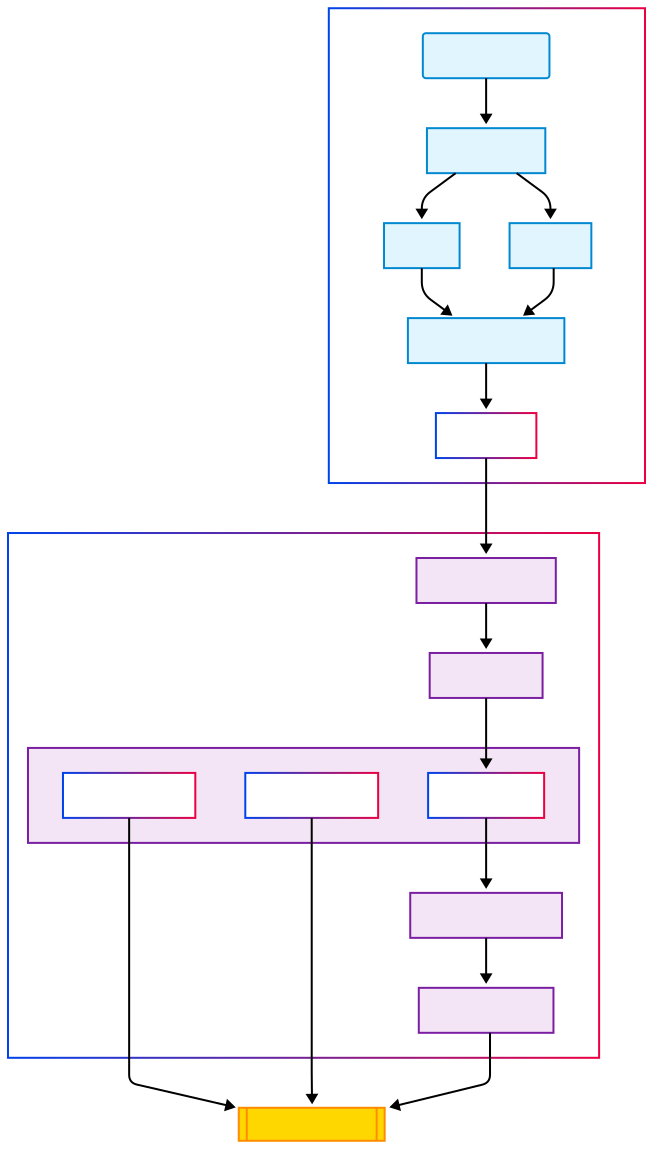
\includegraphics[width=0.85\textwidth]{img/user-diagram-flow}
\caption{High level workflow showing user interaction and data processing}
  \label{fig:user-flow}
\end{figure}

\subsection{Evaluation Framework}\label{subsec:evaluation-framework}
The evaluation framework was designed to combine standardized assessment criteria with carefully crafted prompts that ensure consistent evaluation results across different pitches. The framework uses four main dimensions that were selected based on venture capital research and startup evaluation best practices. Specific weights were assigned to each dimension based on their relative importance in startup success, with the most critical factors receiving higher weights.

The evaluation was structured around these four dimensions with their corresponding weights:

\begin{itemize}
  \item \textbf{Problem\mbox{-}Solution Fit} (0.30)
  \item \textbf{Business Model \& Market} (0.30)
  \item \textbf{Team \& Execution} (0.25)
  \item \textbf{Pitch Quality} (0.15)
\end{itemize}

Problem-Solution Fit and Business Model \& Market were weighted most heavily because these factors are typically the strongest predictors of startup success according to entrepreneurship research. Team \& Execution receives the next highest weight since execution capability is crucial for turning ideas into successful businesses. The lowest weight was assigned to Pitch Quality because while presentation skills matter for raising capital, they are less predictive of actual business success than the fundamental business factors.

Each dimension evaluates five specific aspects and produces both a numeric score and qualitative feedback including strengths and areas for improvement. Table~\ref{tab:criteria} summarizes the detailed criteria and aspects that were implemented for each evaluation dimension.

These evaluation criteria were implemented as structured constants in the system code to ensure consistent application across all pitch assessments. Listing~\ref{lst:eval-criteria} shows the precise criteria and aspect definitions coded into the evaluation system.

\begin{lstlisting}[
  language=JavaScript,
  caption={Evaluation criteria and weights implementation},
  label=lst:eval-criteria,
  basicstyle=\footnotesize\ttfamily,
  breaklines=true
]
const EVALUATION_CRITERIA = {
  problemSolution: {
    name: "Problem-Solution Fit",
    aspects: [
      "Problem Definition Clarity",
      "Solution Innovation",
      "Market Understanding",
      "Competitive Advantage",
      "Value Proposition",
    ],
  },
  businessModel: {
    name: "Business Model & Market",
    aspects: [
      "Revenue Model",
      "Market Size & Growth",
      "Go-to-Market Strategy",
      "Customer Acquisition",
      "Scalability Potential",
    ],
  },
  team: {
    name: "Team & Execution",
    aspects: [
      "Team Capability",
      "Domain Expertise",
      "Track Record",
      "Resource Management",
      "Implementation Plan",
    ],
  },
  presentation: {
    name: "Pitch Quality",
    aspects: [
      "Clarity & Structure",
      "Data & Evidence",
      "Story & Engagement",
      "Q&A Performance",
      "Overall Persuasiveness",
    ],
  },
} as const;

const WEIGHTS: Record<string, number> = {
  "Problem-Solution Fit": 0.3,
  "Business Model & Market": 0.3,
  "Team & Execution": 0.25,
  "Pitch Quality": 0.15,
};
\end{lstlisting}

This code implementation ensures that every evaluation follows exactly the same criteria structure and weighting scheme. The criteria were defined as TypeScript constants to prevent runtime modifications and ensure consistent evaluation behavior. The system processes each criterion separately using these aspect definitions, then combines the results using the specified weights to calculate final scores.

\begin{table}[H]
  \centering
  \caption{Evaluation criteria and aspects (summary)}
  \label{tab:criteria}
  \begin{tabular}{p{4cm} p{9cm}}
    \toprule
    \textbf{Criterion} & \textbf{Aspects} \\
    \midrule
    Problem\mbox{-}Solution Fit & Problem definition clarity; solution innovation; market understanding; competitive advantage; value proposition \\
    Business Model \& Market & Revenue model; market size \& growth; go-to-market strategy; customer acquisition; scalability potential \\
    Team \& Execution & Team capability; domain expertise; track record; resource management; implementation plan \\
    Pitch Quality & Clarity \& structure; data \& evidence; story \& engagement; Q\&A performance; overall persuasiveness \\
    \bottomrule
  \end{tabular}
\end{table}

Figure~\ref{fig:eval-flow} illustrates the four-dimensional processing flow implemented in the system. This diagram shows how each pitch moves through the evaluation pipeline, with the GPT-4 model analyzing the content against each dimension's specific criteria. This single-provider evaluation approach was designed to ensure consistency across all assessments while maintaining the ability to trace how each final score was calculated.

The use of fixed criteria and weights ensures that all evaluation results follow the same methodology, which enables meaningful comparisons between different pitches and supports reproducible research findings.

Specific rubric anchors and scoring rules were designed to address the central tendency problem observed in early testing. These implementation details ensure consistent score distributions and evidence-based assessments. Listing~\ref{lst:scoring-rules} shows the exact rubric anchors and scoring methodology implemented.

\begin{lstlisting}[
  language=JavaScript,
  caption={Rubric anchors and scoring rules implementation},
  label=lst:scoring-rules,
  basicstyle=\footnotesize\ttfamily,
  breaklines=true
]
export const RUBRIC_ANCHORS = `Rubric anchors (apply to every aspect):
1-2: no concrete evidence; claims only
3-4: weak/indirect evidence; plan not validated
5-6: mixed evidence; partial validation or unclear metrics
7-8: strong evidence; credible metrics; risks addressed
9-10: exceptional evidence; repeated traction; benchmarks exceeded`;

export const SCORING_RULES = `Scoring rules:
- Start with aspect scoring; compute the criterion "score" as the 
  rounded average of aspect scores.
- If there are no numbers or specific evidence for an aspect, cap it 
  at 4 and note the gap in the rationale.
- Avoid mid-scale defaults; justify any mid-scale scores against the 
  rubric anchors.`;

export const SCORING_SYSTEM_PROMPT = 
  "You are an experienced venture capitalist. Follow the rubric strictly, " +
  "return valid JSON only, and avoid unsupported claims. Use the full " +
  "1-10 scale based on evidence.";

// Model configuration constants
export const MODEL_NAME = "gpt-4";
export const SCORING_TEMPERATURE = 0.2; // low variance for scoring
export const PROMPT_VERSION = "criteria-v1.2"; // rubric anchors + evidence gating
\end{lstlisting}

These scoring rules solve the central tendency problem by requiring evidence for higher scores and preventing unsupported mid-scale defaults. The evidence threshold was set at score 4, meaning pitches without concrete supporting data cannot score above this level regardless of how well-written their claims might be. The low temperature setting of 0.2 reduces randomness in scoring decisions, improving consistency between evaluations of the same content.

\begin{figure}[H]
  \centering
  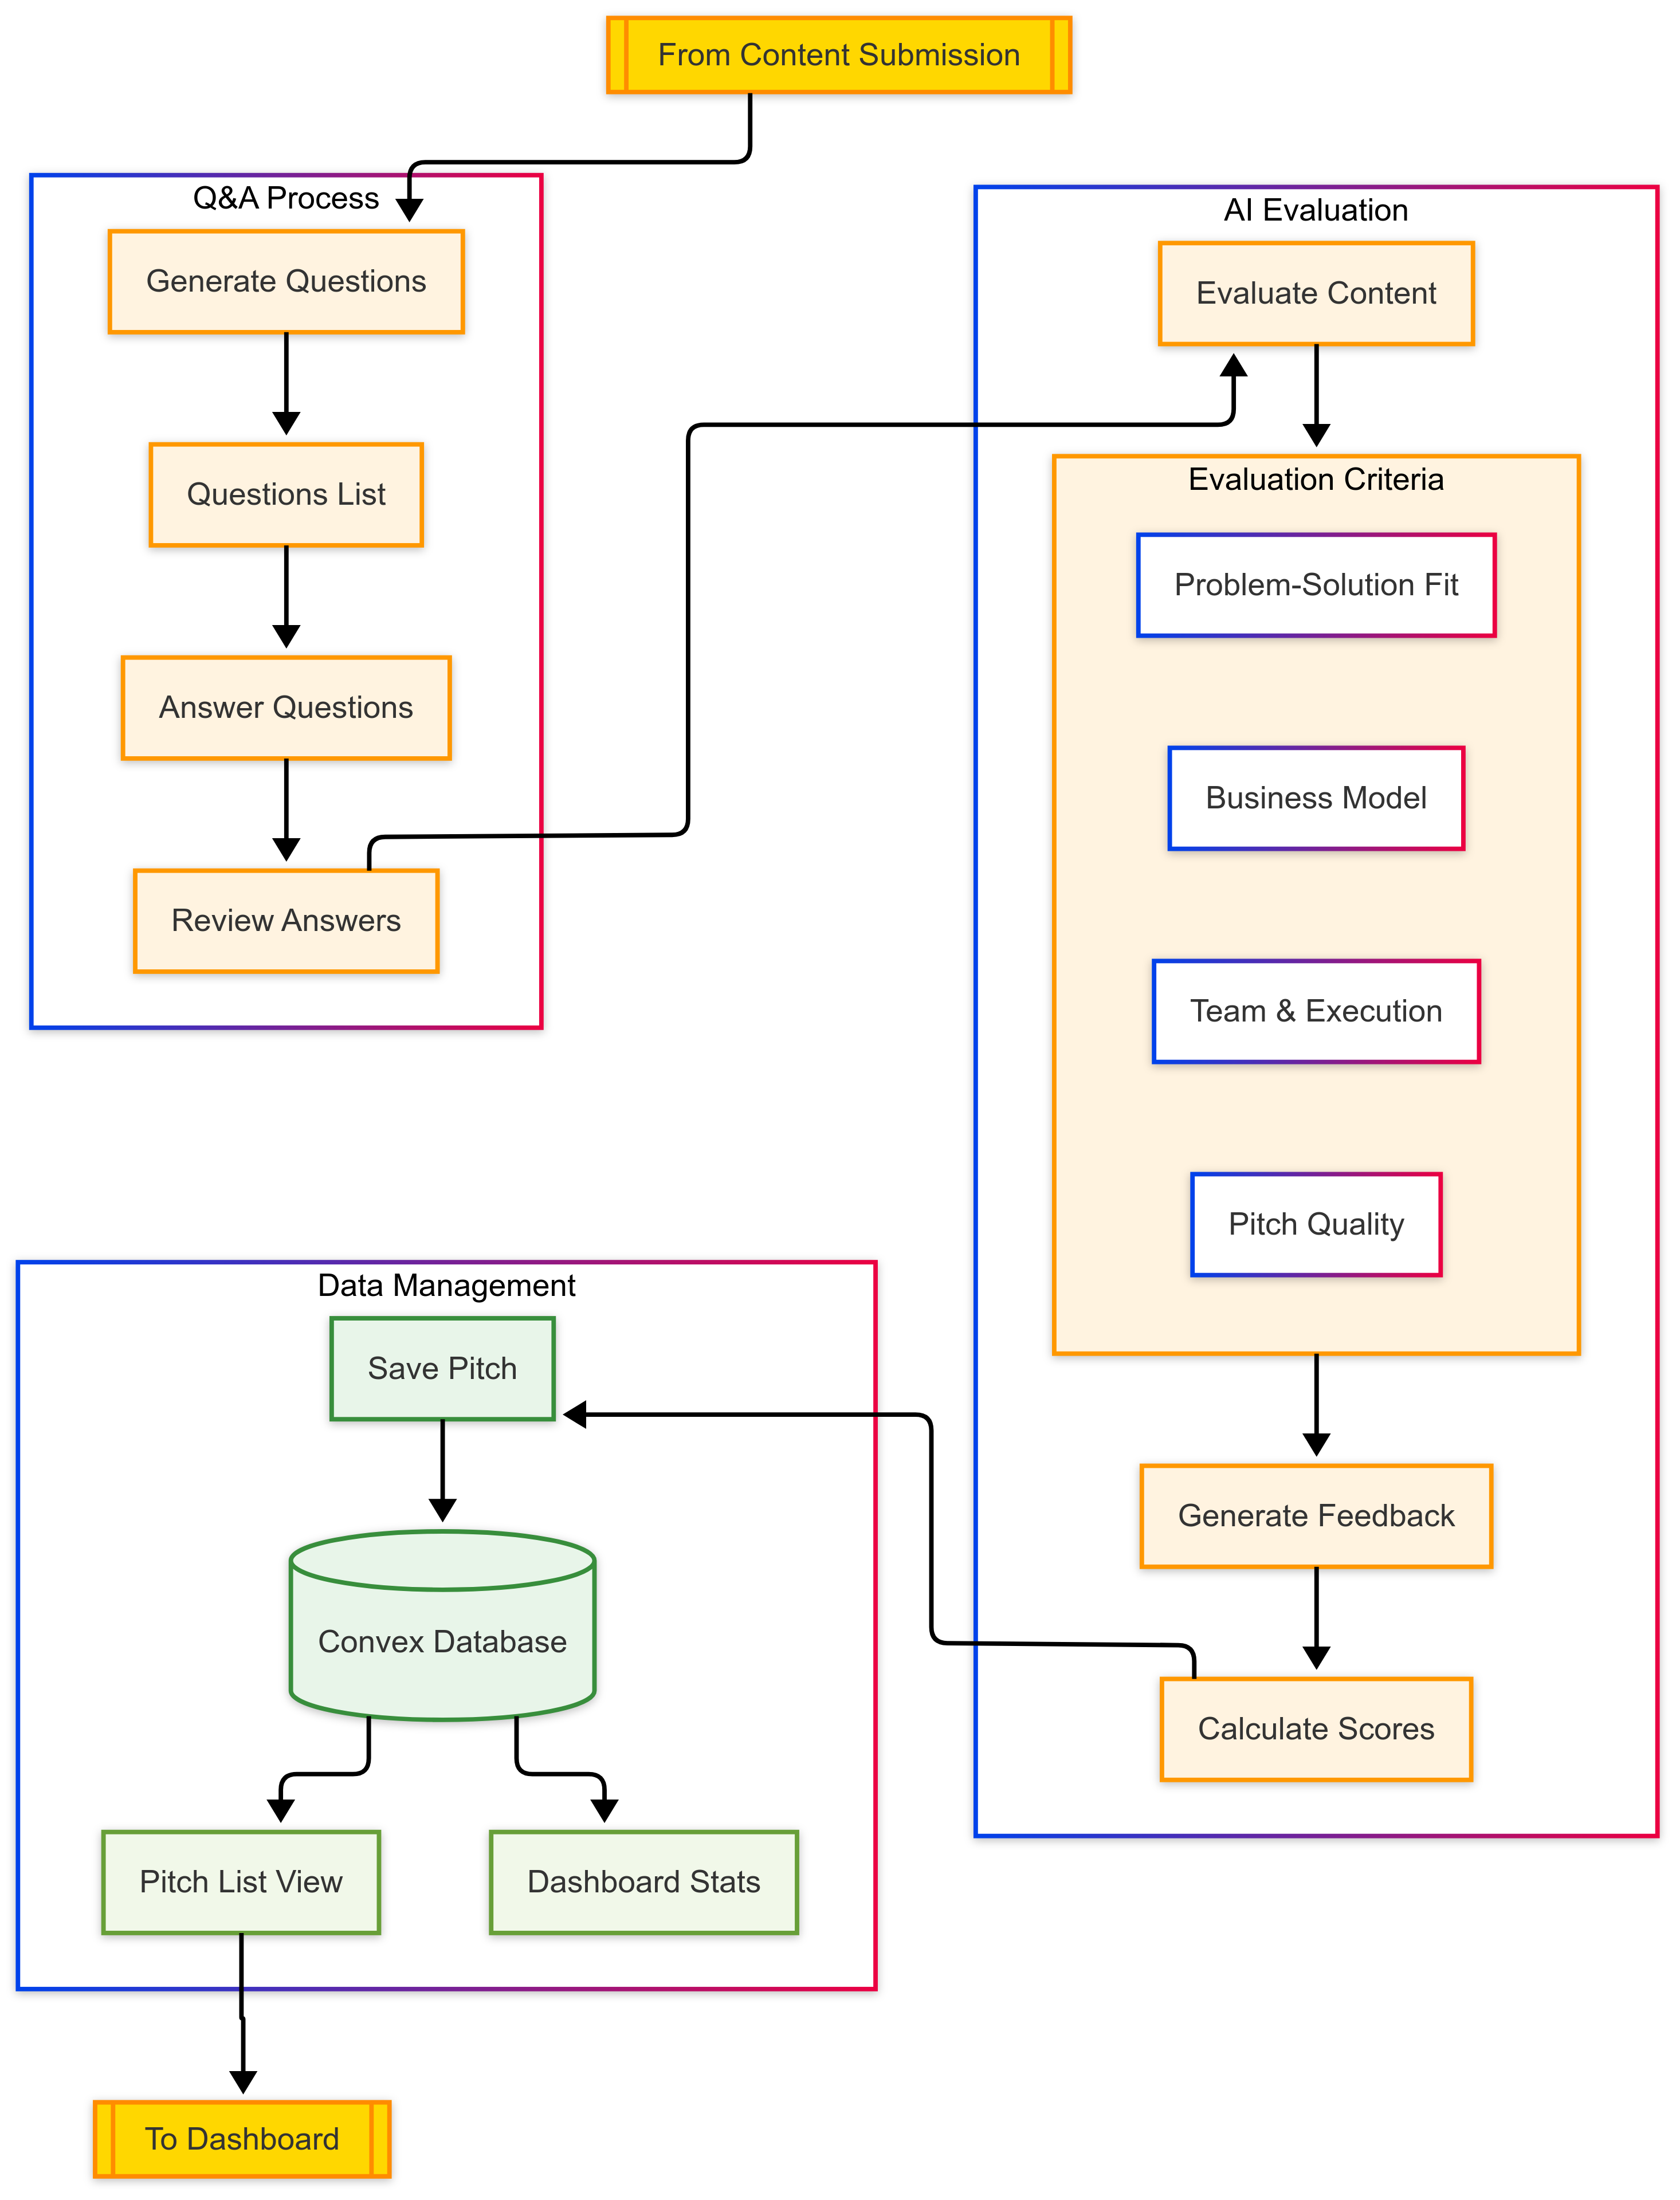
\includegraphics[width=0.9\textwidth]{img/eval-flow}
\caption{Evaluation and processing flow across four criteria}
  \label{fig:eval-flow}
\end{figure}

\subsection{AI Integration Strategy}\label{subsec:ai-integration-strategy}
GPT-4 was integrated through OpenAI's API as the core evaluation engine for Pista after evaluating several large language model options. The system was designed to use structured prompts that return constrained JSON responses, which ensures reliable parsing and consistent data formatting across all evaluations. A single-provider approach was adopted instead of ensemble evaluation or multi-provider systems due to its architectural simplicity while maintaining consistent results. This design enables focus on optimizing one evaluation pathway thoroughly rather than managing multiple competing assessments.

During development, initial evaluations showed a problematic central tendency, with most scores clustering around 7 out of 10. This issue was addressed through a systematic prompt calibration process that improved both the distribution and validity of evaluation scores. Specific rubric anchors were added for the 1-10 scale that clearly define what each score level represents, which helps the model differentiate between pitches of different quality levels. Evidence gating was implemented that caps aspect scores at 4 when specific supporting details are missing from the pitch content, ensuring that higher scores require substantive evidence.

The scoring methodology evaluates individual aspects first and then computes each criterion score as the rounded average of its component aspects. The system was configured to use a lower sampling temperature for scoring requests, which reduces randomness and improves consistency between evaluations of the same content. The current prompt configuration is tracked as \texttt{PROMPT\_VERSION = criteria\textrm{-}v1.2} and this version information is recorded in all evaluation metadata to ensure reproducibility and enable future refinements.

The core evaluation prompt was designed to ensure consistent, evidence-based assessments across all criteria. The implemented prompt structure guides GPT-4 through a systematic evaluation process that prevents unsupported claims and enforces the scoring rubric. Listing~\ref{lst:main-eval-prompt} shows the main evaluation prompt template created for each criterion.

\begin{lstlisting}[
  language=JavaScript,
  caption={Main evaluation prompt template for structured assessment},
  label=lst:main-eval-prompt,
  basicstyle=\footnotesize\ttfamily,
  breaklines=true
]
function buildStructuredPrompt(
  criteriaName: string,
  aspects: string[],
  fullContent: string
): string {
  return `
As an expert evaluator, score ONLY the criterion: ${criteriaName}.

Work from the content below without inventing facts. If evidence is 
missing for an aspect, score that aspect <= 4 and note what is missing.

Aspects to score (each 1-10 with a one sentence rationale):
${aspects.map((aspect) => `- ${aspect}`).join("\n")}

Content to evaluate (pitch + Q&A):
${fullContent}

${RUBRIC_ANCHORS}

JSON response schema (valid JSON only):
{
  "score": 1-10, // criterion score = rounded average of aspectScores[].score
  "strengths": [{ "point": "...", "impact": "High"|"Medium"|"Low"}],
  "improvements": [{ "area": "...", "priority": "Critical"|"Important"|"Nice to Have", "actionable": "..."}],
  "aspectScores": [
    { "aspect": "${aspects[0]}", "score": 1-10, "rationale": "..." },
    { "aspect": "${aspects[1]}", "score": 1-10, "rationale": "..." },
    { "aspect": "${aspects[2]}", "score": 1-10, "rationale": "..." },
    { "aspect": "${aspects[3]}", "score": 1-10, "rationale": "..." },
    { "aspect": "${aspects[4]}", "score": 1-10, "rationale": "..." }
  ],
  "summary": "2-3 sentence synthesis",
  "recommendations": ["actionable step 1", "actionable step 2"]
}

${SCORING_RULES}
`;
}
\end{lstlisting}

This prompt template enforces evidence-based evaluation by explicitly instructing the model to avoid inventing facts and to cap scores at 4 when supporting evidence is missing. The prompt was structured to require JSON responses with specific fields for strengths, improvements, and detailed aspect-level scoring with rationales. The template ensures consistent evaluation across all four criteria while maintaining the flexibility needed for different types of startup pitches.

A separate question generation system was also developed to gather additional evidence before conducting the main evaluation. The question generation prompt focuses on identifying the most important information gaps that could materially impact the assessment quality. Listing~\ref{lst:question-prompt} shows the question generation prompt implemented.

\begin{lstlisting}[
  language=JavaScript,
  caption={Question generation prompt for evidence gathering},
  label=lst:question-prompt,
  basicstyle=\footnotesize\ttfamily,
  breaklines=true
]
const prompt = [
  `Analyze the following pitch and identify the most important gaps that prevent a confident evaluation. Select up to 3 questions that, if answered, would materially improve the assessment.`,
  `Pitch:\n"${truncate(text, MAX_PROMPT_CHARS)}"`,
  `\nReturn valid JSON only with this schema:\n{\n  "items": [\n    {\n      "dimension": "Problem-Solution Fit" | "Business Model & Market" | "Team & Execution" | "Pitch Quality",\n      "question": "one specific question, no multi-part prompts",\n      "why_needed": "why this matters for evaluation",\n      "suggested_format": "how to answer: numbers, metrics, bullets, examples",\n      "priority": "Critical" | "Important"\n    }\n  ]\n}\n\nConstraints:\n- Ask 1–3 questions total.\n- Make each question specific and evidence-seeking.\n- Do not request sensitive data (PII, secrets, internal docs).\n- Avoid duplicates and multi-part questions.`,
].join("\n\n");

const QUESTION_SYSTEM_PROMPT = `You are an experienced venture capitalist. Ask only the highest-priority follow-up questions that close information gaps. Questions must be specific, evidence-seeking, and answerable by a typical pitch. Return valid JSON only.`;
\end{lstlisting}

This question generation approach systematically identifies evidence gaps across the four evaluation dimensions before conducting the final assessment. The prompt was designed to prioritize questions that would have the highest impact on evaluation accuracy while ensuring the questions remain answerable within a typical pitch context. The structured JSON response format allows the system to tag each question to its corresponding evaluation dimension, ensuring comprehensive coverage of all assessment criteria.

Robust error handling was implemented for all OpenAI API interactions using retries with exponential backoff to manage rate limits and transient network failures. The system validates all API responses against strict application schemas before persisting any evaluation data, which prevents corrupted or malformed evaluations from entering the database.

\subsection{Data Models and Storage Architecture}\label{subsec:data-models-and-storage-architecture}
The data storage architecture was designed using Convex to provide both robust data persistence and real-time user interface updates without the complexity of traditional database management. Convex was chosen because it combines database functionality with built-in schema validation and indexed access patterns, which simplifies development while ensuring data integrity. A multi-tenant architecture was implemented where each document is automatically scoped by user and organization identifiers, providing secure data isolation without requiring complex authorization logic.

The data model stores question-and-answer pairs with each pitch and reuses this information when building evaluation input, which allows the system to gather additional context that improves assessment quality. The system was designed so that user interface queries update reactively whenever underlying data changes, eliminating the need for manual polling or refresh operations. This approach provides a responsive user experience where evaluation results appear immediately after processing completes.

The main \texttt{pitches} table was structured to store essential pitch information including title, normalized text content, submission type, and processing status. The table also persists structured evaluation results, question-and-answer pairs, organization identifiers, user identifiers, author names, and creation timestamps. Several database indexes were implemented including \texttt{by\_org}, \texttt{by\_user}, \texttt{by\_user\_org}, and \texttt{search\_title} to support efficient queries for different access patterns. A separate \texttt{userFavorites} table was also created that links users and pitches through composite indexes, allowing users to bookmark pitches of interest without affecting the main pitch data.

\subsection{API Endpoints and Server Functions}\label{subsec:api-and-server}
The system's API architecture was designed to separate concerns between Next.js API routes that handle AI processing and Convex functions that manage data persistence and retrieval. This separation allows each component to be optimized for its specific purpose while maintaining clean interfaces between different system layers.

Several Next.js API routes were implemented that handle the AI-powered processing components of the evaluation pipeline. The \texttt{/api/evaluate} endpoint processes pitch text using GPT-4 and runs on the Edge runtime for improved performance and global distribution. The \texttt{/api/generate-questions} endpoint was created to produce up to three follow-up questions that help gather additional evidence for evaluation. An \texttt{/api/evaluate-answers} endpoint was also built that can update evaluations based on question responses, though this was not used in the primary user interface flow to keep the process streamlined. The \texttt{/api/transcribe} endpoint handles audio file transcription using OpenAI's Whisper model\footnote{\url{https://openai.com/research/whisper}}, which enables the system to process pitch videos and audio recordings.

Several Convex functions were developed in \texttt{convex/pitches.ts} that handle all data operations for the application. The mutation functions include \texttt{create}, \texttt{update}, \texttt{remove}, \texttt{favorite}, \texttt{unfavorite}, and \texttt{prefetch}, which cover all the data modification operations users can perform. Query functions were implemented including \texttt{get}, \texttt{getPitch}, \texttt{getFilteredPitches}, \texttt{getPitchStats}, and \texttt{exportCSV} to support different data access patterns needed by the user interface.

The question generation system was designed to request one to three high-priority, evidence-seeking questions that target specific gaps in the original pitch content. The system returns a structured JSON response where each question is tagged to a specific evaluation dimension, which helps ensure comprehensive coverage of all assessment criteria. This endpoint was configured to use a lower sampling temperature for improved stability and consistency in question generation. A fallback parser was also implemented that can extract questions from plain text responses if the model doesn't return properly formatted JSON, which makes the system more robust to variations in AI model behavior. This question generation approach improves evidence capture for the calibrated scoring rubric without modifying the original pitch content.

The complete evaluation pipeline follows a clear sequence: transcribe audio content if needed, generate targeted questions, collect answers, perform comprehensive evaluation, and store results in the database.

Precise TypeScript interfaces were defined to ensure consistent data structures across all API responses and database storage. These type definitions enforce the structured evaluation format and prevent data inconsistencies during processing. Listing~\ref{lst:response-schema} shows the key response schema types implemented for the evaluation system.

\begin{lstlisting}[
  language=TypeScript,
  caption={Structured evaluation response schema types},
  label=lst:response-schema,
  basicstyle=\footnotesize\ttfamily,
  breaklines=true
]
export interface StructuredEvaluation {
  criteria: string;
  score: number;
  breakdown: {
    strengths: Array<{
      point: string;
      impact: "High" | "Medium" | "Low";
    }>;
    improvements: Array<{
      area: string;
      priority: "Critical" | "Important" | "Nice to Have";
      actionable: string;
    }>;
    aspectScores: Array<{
      aspect: string;
      score: number;
      rationale: string;
    }>;
  };
  summary: string;
  recommendations: string[];
}

export interface StructuredEvaluationData {
  evaluations: StructuredEvaluation[];
  overallScore: number;
  overallFeedback: StructuredFeedback;
  metadata: {
    evaluatedAt: string;
    modelVersion: string;
    processingTime?: number;
    promptVersion?: string;
    policyVersion?: string;
  };
}

export interface StructuredFeedback {
  overallAssessment: {
    summary: string;
    keyHighlights: string[];
    primaryConcerns: string[];
  };
  investmentThesis: {
    viability: "Strong" | "Moderate" | "Weak" | "Not Applicable";
    reasoning: string;
    potentialReturns: string;
  };
  riskAssessment: {
    majorRisks: Array<{
      risk: string;
      severity: "High" | "Medium" | "Low";
      mitigation: string;
    }>;
    riskScore: number; // 1-10, lower is better
  };
  // Additional fields: nextSteps, competitivePosition, foundersAssessment
}
\end{lstlisting}

These TypeScript interfaces enforce strict typing throughout the evaluation system, preventing runtime errors and ensuring consistent data structures. The schema was designed to capture both quantitative scores and qualitative feedback at multiple levels of detail, from individual aspect rationales to comprehensive investment assessments. The metadata fields track evaluation timestamps, model versions, and processing times, which supports reproducibility and system monitoring for research applications.

\section{Authentication and Authorization Implementation}

Authentication and authorization were implemented using Clerk to handle user sign-in, session management, and organization contexts throughout the application. Clerk was chosen because it provides complete authentication infrastructure without requiring the building and maintenance of complex user management systems. The service handles password security, email verification, multi-factor authentication, and organization management features that would take significant development time to implement correctly.

Next.js middleware was configured to protect application routes and inject user identity information on the server side, which ensures that only authenticated users can access the evaluation system. The authorization model was designed using row-level scoping where all Convex database reads and writes are automatically filtered by \texttt{userId} and \texttt{orgId} parameters. This approach provides complete data isolation between different users and organizations without requiring the implementation of custom role-based access control systems or management of complex permission tables. The scoping happens automatically at the database query level, which prevents data leakage and simplifies the security model.

Middleware route protection combined with database-level row scoping enforces secure data isolation without complex role management systems.

\section{User Interface Implementation}

The user interface was designed to provide an intuitive and efficient experience for users evaluating startup pitches while maintaining the consistency needed for research applications. Next.js 15 with React 18 and Tailwind CSS\footnote{\url{https://tailwindcss.com}} was chosen as the frontend technology stack because it enables rapid development of responsive interfaces with modern user experience patterns. The application was organized using Next.js route groups that separate the interface into distinct areas: dashboard for pitch management, individual pitch pages for detailed evaluation views, and authentication areas for user management.

The component architecture was structured to promote reusability and maintainability by separating shared UI primitives under \texttt{src/components/ui} from feature-specific components under \texttt{src/components/shared}. This organization allows consistent design patterns to be maintained while building complex user interface functionality. Comprehensive list management features were implemented that support user favorites, text-based search, and filtering by evaluation scores or submission dates. The individual pitch view renders both numeric scores and qualitative feedback alongside the generated follow-up questions, providing users with complete evaluation information in a clear, structured format.

Figure~\ref{fig:user-flow-pitch} illustrates the pitch creation flow designed to guide users through the evaluation process systematically. The flow handles both text input and audio file uploads, manages question generation and response collection, performs evaluation processing, and stores results in the Convex database. The question-and-answer step was made mandatory in production use because it significantly improves evaluation quality by capturing evidence that might be missing from the original pitch content. This requirement ensures that all evaluations benefit from the additional context gathering that improves scoring accuracy.

\begin{figure}[H]
  \centering
  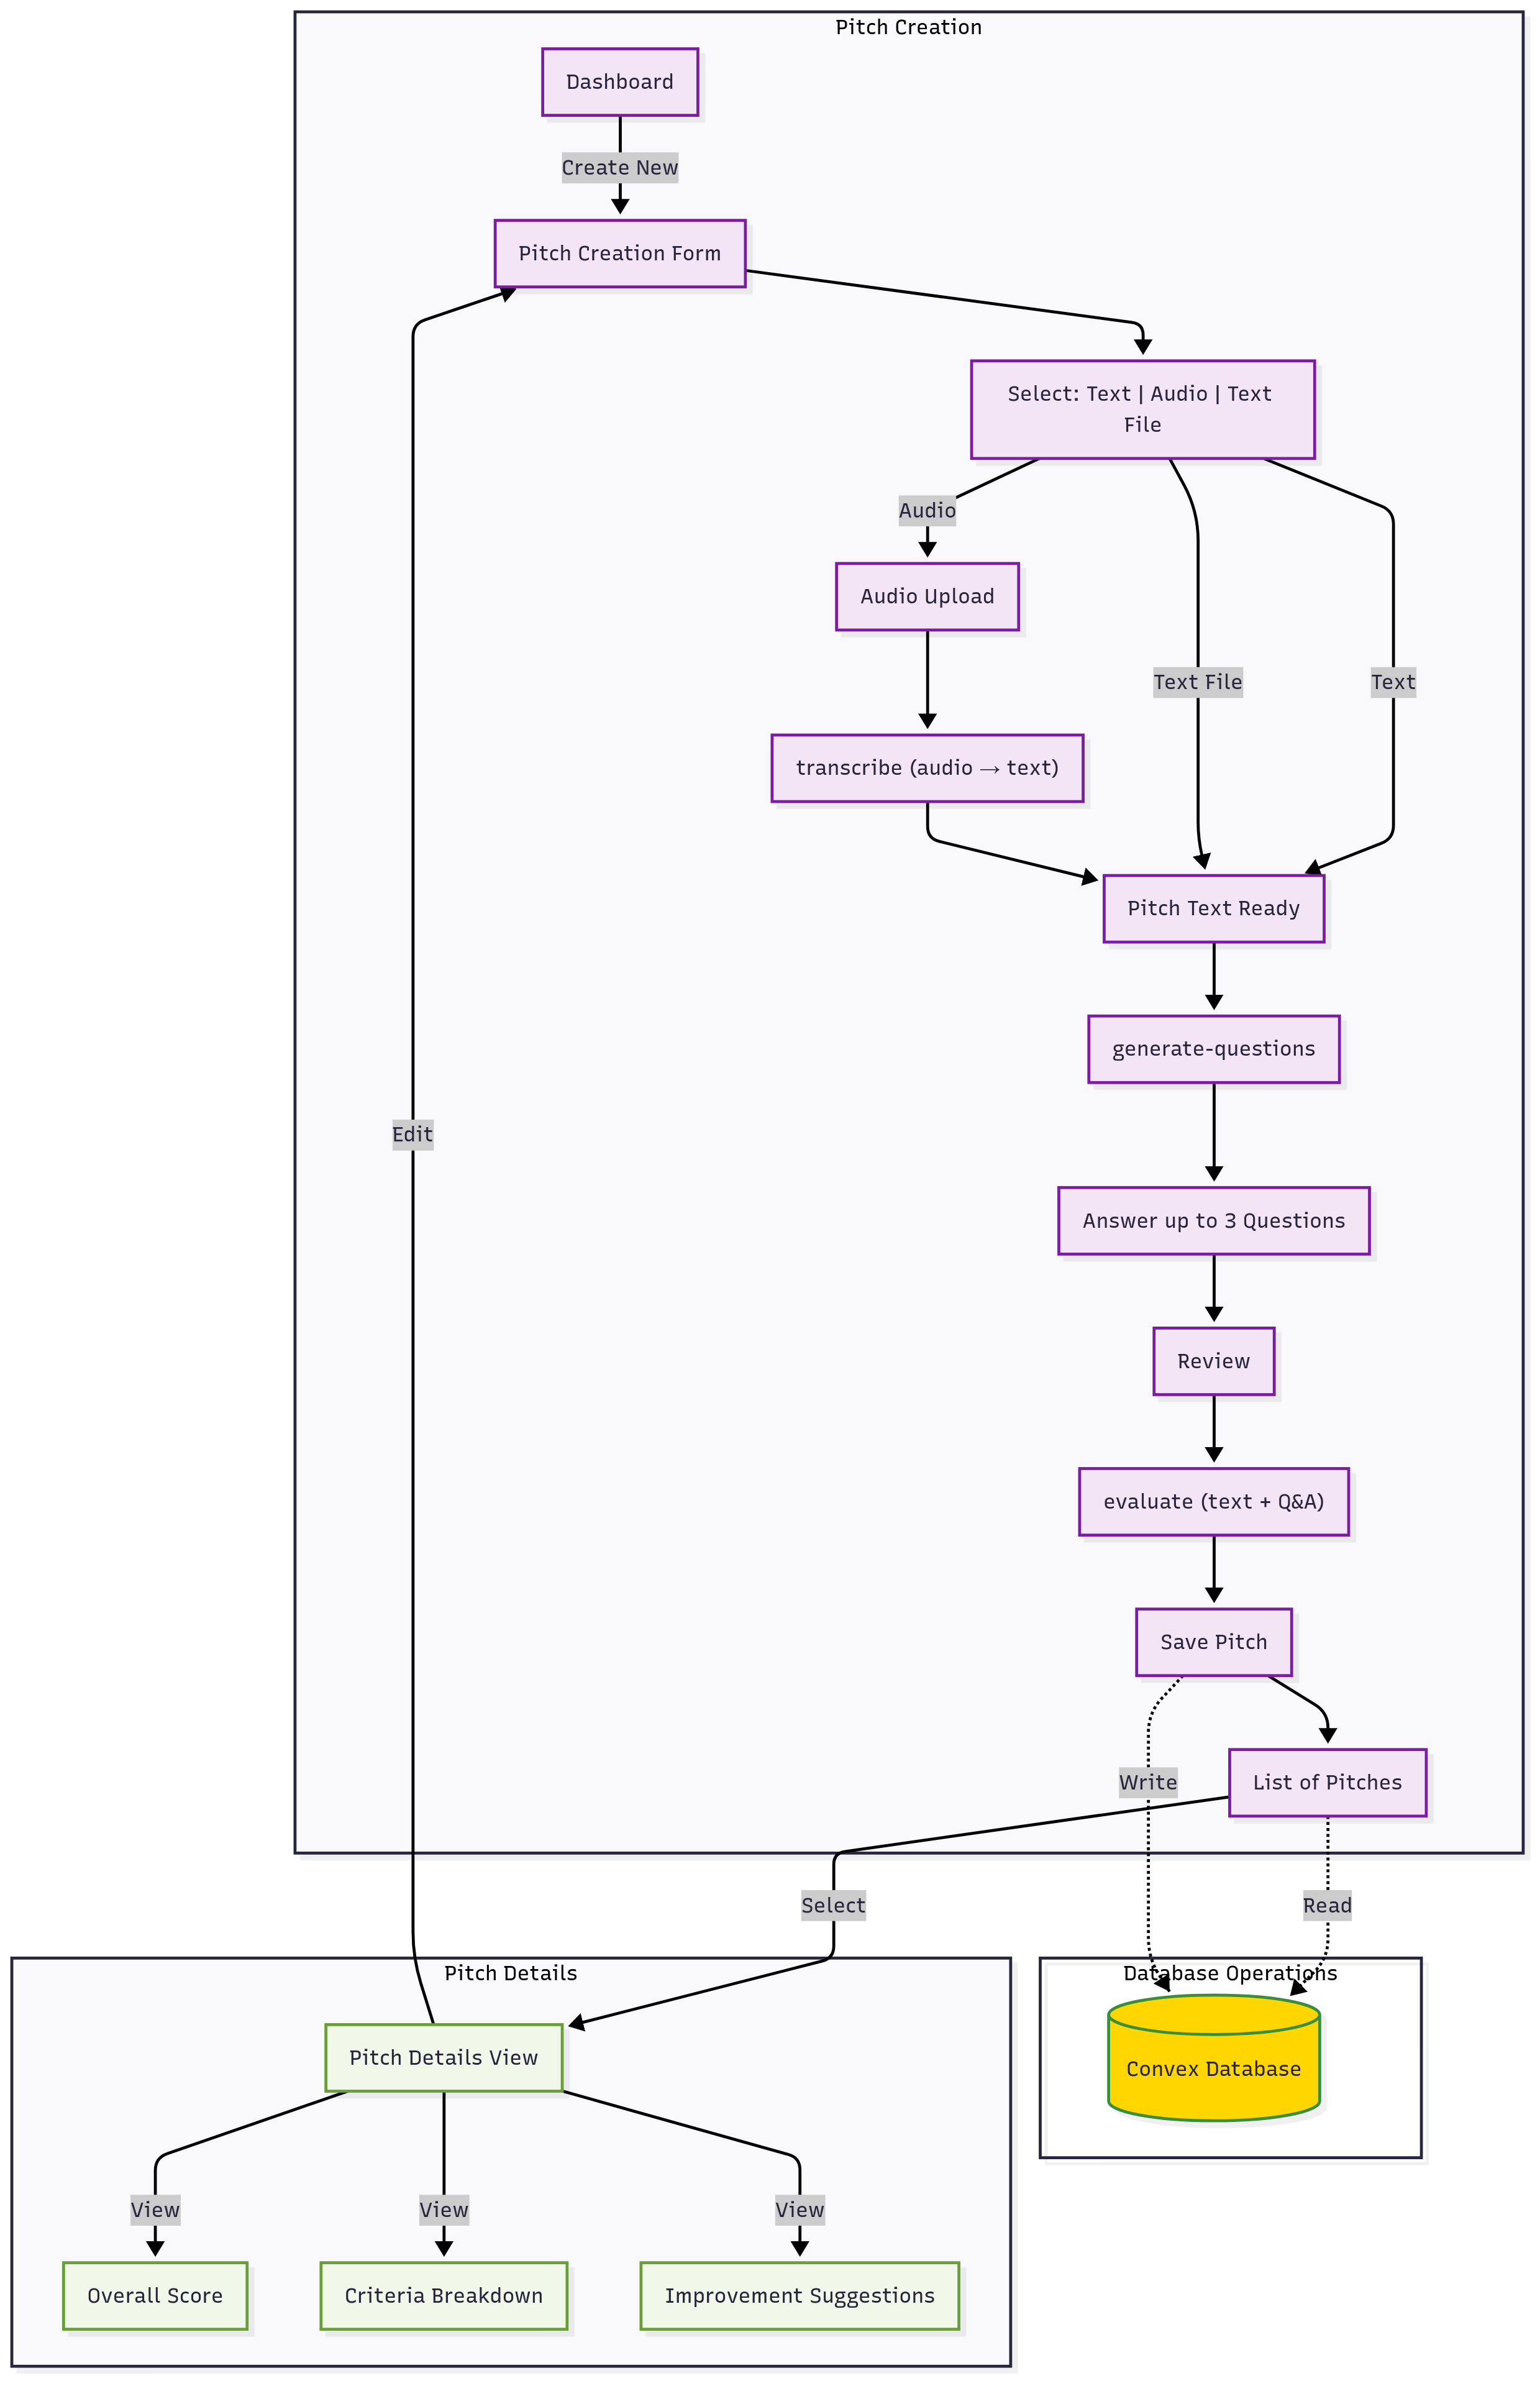
\includegraphics[width=0.9\textwidth]{img/user-flow-pitch}
\caption{Pitch creation flow with Q\&A generation and Convex storage}
  \label{fig:user-flow-pitch}
\end{figure}

The user interface guides users through a streamlined, consistent evaluation process while presenting comprehensive scores and feedback in an accessible format.

\section{Performance, Deployment, and Reliability}

The system's performance characteristics were designed to handle the computational demands of AI-powered evaluation while maintaining responsive user interactions. Virtualized lists were implemented that keep the interface responsive even when users work with large datasets of evaluated pitches. Code splitting techniques were used to defer loading of non-critical user interface components, which reduces initial page load times and improves the perceived performance of the application. The reactive query system eliminates manual polling by automatically updating the interface when evaluation results become available, which provides immediate feedback to users without requiring page refreshes.

The deployment architecture was configured to optimize both performance and reliability across different environments. Critical API routes run on Vercel's Edge runtime where configured, which provides global distribution and reduced latency for evaluation requests. System configuration is managed through environment variables including the Convex database URL, Clerk authentication keys, and OpenAI API credentials. Identical code paths were ensured to execute in both development and production environments, which maintains comparability of evaluation results across different deployment contexts and enables reliable testing of system behavior.

Comprehensive error handling and reliability measures were implemented throughout the system architecture. API routes return clear, actionable error messages that help users understand what went wrong and how to resolve issues without exposing sensitive internal system details. The user interface presents error information in a way that guides users toward successful task completion while maintaining security by not revealing system internals that could be exploited.

Performance optimizations and deployment strategies prioritize system responsiveness and maintain consistent behavior across all environments.

\section{Implementation Results and User Experience}\label{sec:results}

The system's performance characteristics and user experience were measured to validate that the implementation meets the design objectives established for responsive and consistent startup pitch evaluation. Text-based pitch evaluations typically complete within 30 to 60 seconds from submission to final results, which provides users with timely feedback without creating lengthy waiting periods. Audio-based submissions require additional processing time for transcription using the Whisper model, but the total evaluation time remains reasonable for practical use in both research and educational contexts.

The user interface was designed to provide immediate visual feedback throughout the evaluation process, with reactive updates that make list changes visible without requiring manual page refreshes. Users can see evaluation progress in real time and access results immediately after processing completes. The system maintains responsive performance even when handling multiple simultaneous evaluations, which supports both individual use and classroom scenarios where multiple students might submit pitches concurrently.

The performance and user experience characteristics demonstrate achievement of the design goals established for creating a system that provides responsive, consistent pitch assessments suitable for academic research and iterative development work. The combination of reasonable processing times, reactive interface updates, and reliable performance enables the system to serve both research and practical evaluation needs effectively.

The implemented Pista system is documented as currently operational. Emphasis was placed on the working system rather than covering earlier experimental approaches with NextAuth and PostgreSQL, industry-specific weight profiles, or ensemble evaluation using multiple model providers. Those alternative approaches represent potential future extensions that are referenced in the discussion chapter as opportunities for continued research and development.
